\documentclass[12pt]{article}

\usepackage{times}
\usepackage{amsmath}
\usepackage{latexsym}
\usepackage{fullpage}
\usepackage{graphicx}
\usepackage{amsfonts}

\graphicspath{ {./images/} }

\newcommand{\NOT}{\neg}
\newcommand{\AND}{\wedge}
\newcommand{\OR}{\vee}
\newcommand{\XOR}{\oplus}
\newcommand{\IMPLIES}{\rightarrow}
\newcommand{\IFF}{\leftrightarrow}
\newcommand{\E}{\exists}
\newcommand{\A}{\forall}

\setlength{\parskip}{.1in}

\renewcommand{\baselinestretch}{1.1}

\begin{document}

\begin{center}

{\bf
CSCE 313\\
PA6-Report\\
Jeffrey Xu\\
11/23/20\\
}

\end{center}

\section{Time Complexity of TCP Connections}

We need to analyze the runtime and time complexity of our PA6 with previous runtimes of PAs. The main difference with this PA and other PAs is that now we are using TCP connections to make patient and file requests. Since this isn't running in the same machine per se, the runtimes can vary dramatically since TCP connections may have different reachabilities and connection speeds. This will give some longer runtimes for some requests compared to just using ICP methods. The plots below give the runtimes for various $w$ and $b$ values for patient requests. 

When testing the workers, we set $b=100$. When testing the bounded buffer size, we set $w=500$ for consistent results. The setup for the server-client for these tests were two separate laptops (separate machines). 

\begin{center}
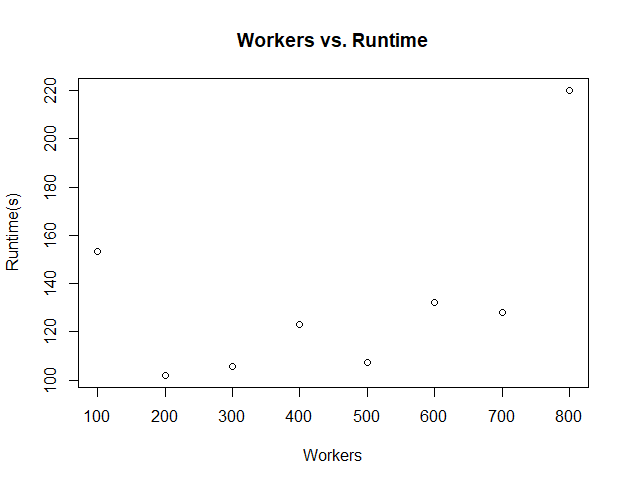
\includegraphics[width=8cm, height=6cm]{PA6_WT}
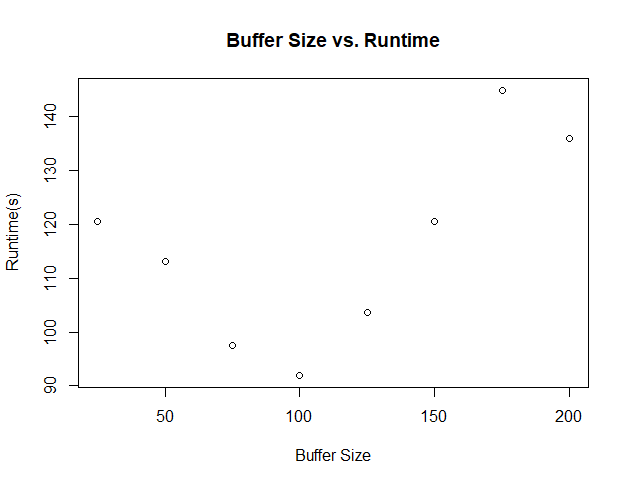
\includegraphics[width=8cm, height=6cm]{PA6BT}
\end{center}

We notice that the worker dimenishing point is around 200-300 now and after that, the runtime slowly begins to increase until it hits 800 workers. This dimenishing point is much lower than the dimenishing point in PA5. This can be attributed to the fact that TCP connections are being used instead of FIFO pipes. The bufer size seems to have an optimal size at around 100 and after that, the runtime begins to increase linearly. 

Comparing with the runtimes of PA5, we notice that PA6 takes significantly longer. The runtimes are almost double the amount of the runtime that was recorded in PA5. This can be attributed to the fact that TCP connections take longer than FIFO pipes and depending on the location and network strength, TCP requests can take different amounts of time. 

PA6 Bonus Demo with Desktop and Laptop Setup: https://youtu.be/bmPp519Yiv0

PA6 Demo: https://youtu.be/wYIWk9Tf1OU

\end{document}